\documentclass[final, usenames, dvipsnames]{beamer}

\title{Real Time Shape Reconstruction for Near Earth Asteroid Landing}
\author{Shankar kulumani}
\year=2018
\subtitle{\the\year~SEAS Student Research and Development Showcase}
\institute{Flight Dynamics and Controls Laboratory (Dr. Taeyoung Lee)\\Department of Mechanical and Aerospace Engineering, School of Engineering and Applied Science}

\mode<presentation>{\usetheme{GWU}}
\usepackage{poster_packages}
\input{my_macros}
\usepackage[orientation=landscape,size=custom,scale=1.32, width=121.92, height=91.44]{beamerposter} 
%\beamertemplategridbackground[0.1in] % grid for aligning stuff

%\setlength{\abovecaptionskip}{0.1cm}
%\setlength{\belowcaptionskip}{-0.3cm}

\def\newblock{} % Avoid the "\newblock undefined" error. See http://newsgroups.derkeiler.com/Archive/Comp/comp.text.tex/2008-07/msg00381.html"

%-----------------------------------------------------------
\newlength{\colsep}
\newlength{\onecolwidth}
\newlength{\twocolwidth}

%\setlength{\onecolwidth}{0.23\textwidth} % Width of one column
%\setlength{\twocolwidth}{0.49\textwidth} % Width of two columns
\setlength{\onecolwidth}{28cm} % Width of one column
\setlength{\twocolwidth}{59cm} % Width of two columns
\newlength{\columnheight}
\setlength{\columnheight}{76.5cm}

\setbeamersize{text margin left=1.5cm,text margin right=0.5cm}

\listfiles

%-----------------------------
% MACROS
%-----------------------------
\def\Emph{\textcolor{RoyalBlue}}

%----------------------------------------------------------------------------------------

\begin{document}
\begin{frame}[t] % enclose entire poster in a frame
\begin{columns}[T,onlytextwidth] % start of all columns in poster

%-----------------------------------------------------------------------------------------
% FIRST (LEFT) COLUMN
%---------------------------------------------------------------------------------------
    \begin{column}{\onecolwidth} % first column start

        \begin{block}{Introduction} % Background block
            \begin{itemize}
                \item Asteroids and comets are of significant interest 
                    \begin{itemize}
                        \item \Emph{Science} - Insight into early solar system formation
                        \item \Emph{Mining} - vast quantities of useful materials
                        \item \Emph{Impact} - high risk from hazardous Near-Earth asteroids
                    \end{itemize}
                \item Near-Earth asteroids (NEAs) are especially interesting 
                    \begin{itemize}
                        \item Orbit close to the Earth and are easily accessible
                        \item Many asteroids hold vast quantities of useful materials
                        \item Asteroid mining: Precious metals, propulsion fuels, semiconductors
                        \item Commercialization is feasible with huge amounts of possible profit 
                    \end{itemize}
                \item High probability of future asteroid impacts
            \end{itemize}
            \vspace{0.2in}
            \begin{figure}
                \centering
                \subcaptionbox{Asteroid Mining\label{fig:ast_mining}}{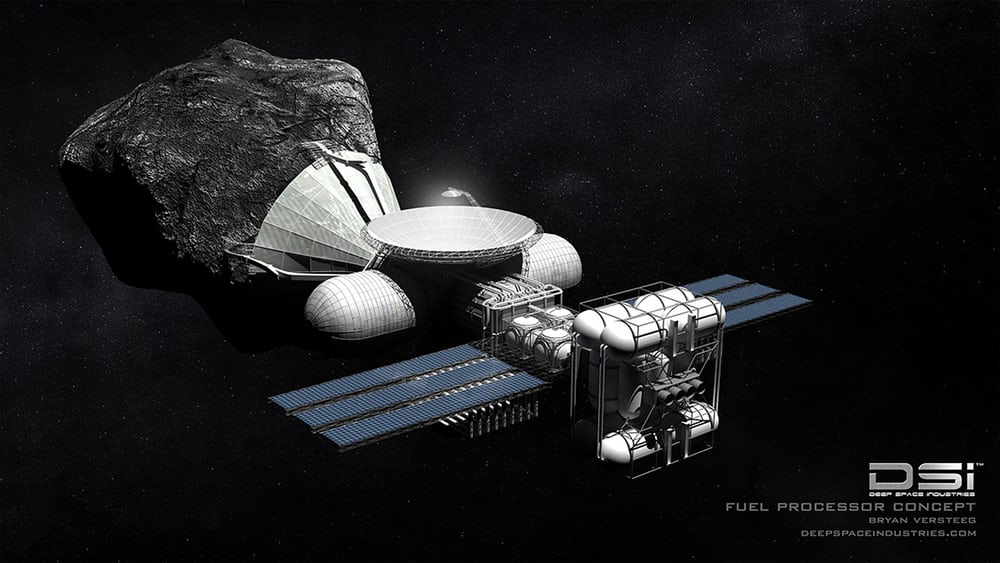
\includegraphics[width=0.4\columnwidth,height=7cm]{figures/asteroid-mining-feature-8.jpg}}~
                \subcaptionbox{Asteroid Impact\label{fig:ast_impact}}{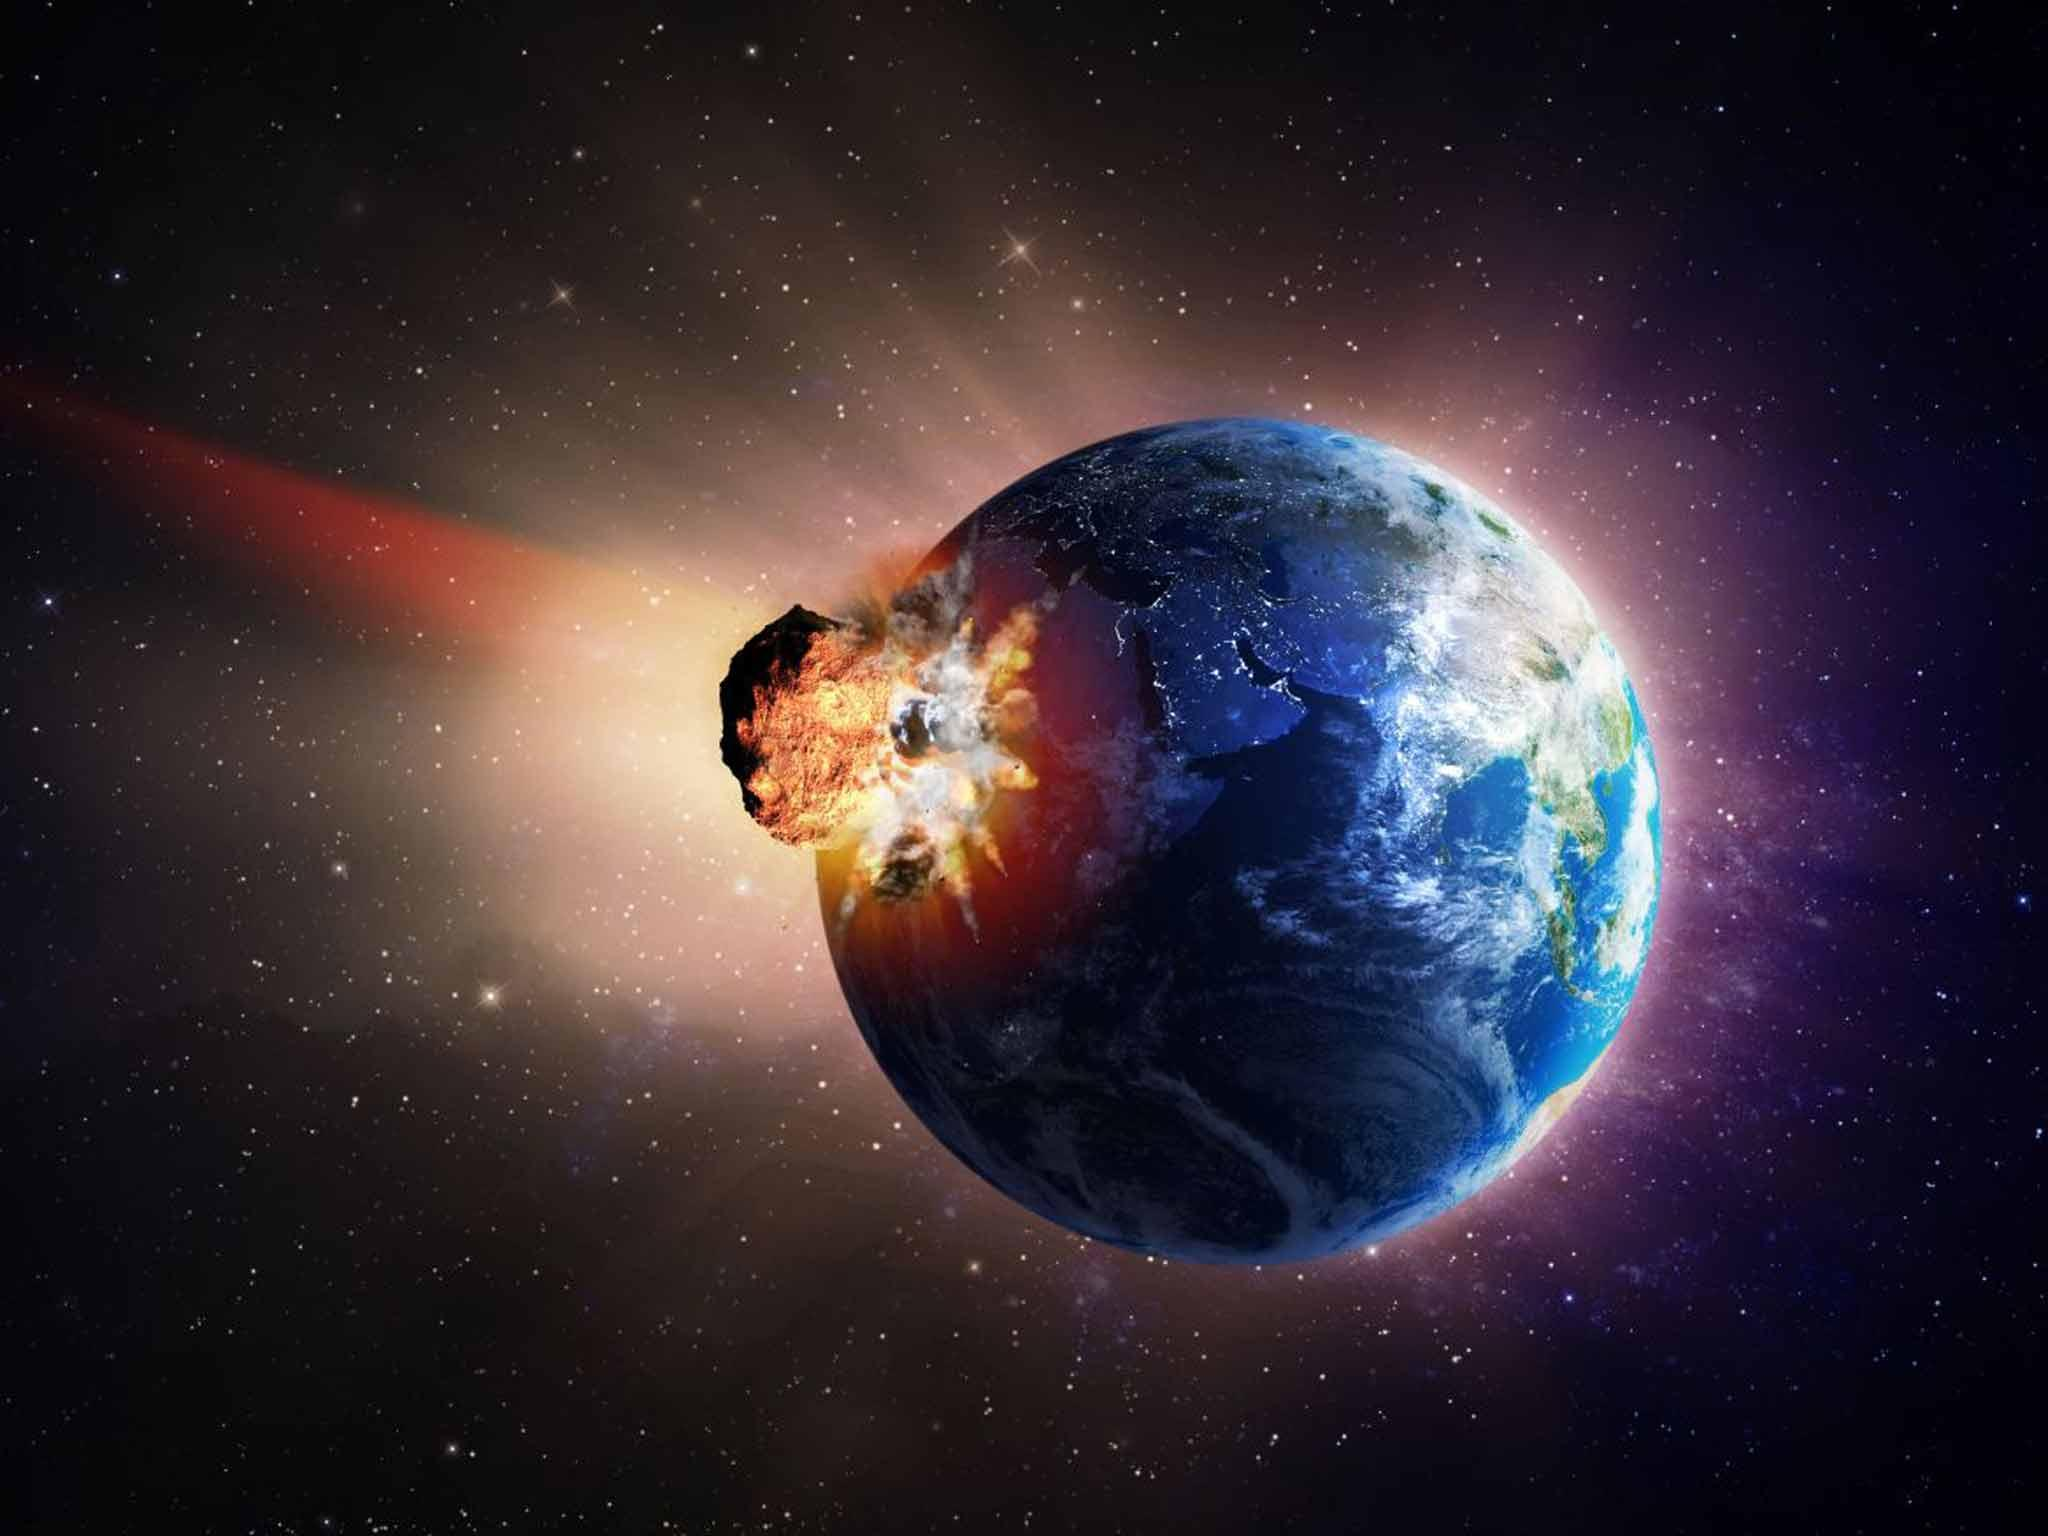
\includegraphics[width=0.4\textwidth,height=7cm,keepaspectratio]{figures/asteroid-alamy.jpg}}
            \end{figure}
        \end{block} % end of background block

        \begin{block}{Technical Challenges}
            \begin{itemize}
                \item Unknown asteroid shape and dynamics
                    \begin{itemize}
                        \item Only a rough estimate of the shape and mass of asteroid is possible from Earth
                        \item At arrival, spacecraft is flying into an unknown environment 
                        \item Spacecraft must autonomously survey the asteroid and handle unknown perturbations
                    \end{itemize}
                \item Optimal trajectory design is complicated
                    \begin{itemize}
                        \item Highly nonlinear and chaotic dynamics requires intuition by designer
                        \item Using low-thrust propulsion adds additional difficulties in accurately capturing the small perturbations
                    \end{itemize}
                \item Astrodynamic trajectory design typically uses direct optimal control
                    \begin{itemize}
                        \item Large nonlinear programming problem inherently approximates the true optimal solution
                        \item High dimensionality of the solution makes it extremely computationally intensive
                    \end{itemize}
            \end{itemize}
        \end{block} 

        \begin{block}{Shape/Gravitational Modeling}
            \begin{itemize}
                \item Asteroids are extended bodies - not point masses
                    \begin{itemize}
                        \item Gravity is the key force in orbital mechanics
                        \item An accurate representation of gravity is critical to accurate and realistic analysis
                    \end{itemize}
                \item \Emph{Polyhedron Gravitational model} used to represent the asteroid
                    \begin{itemize}
                        \item Globally valid and closed-form analytical solution for gravity
                        \item Exact potential assumes a constant density assumption
                        \item Accuracy is only dependent on the shape
                    \end{itemize}
                    \[
                        U(\vecbf{r}) = \frac{1}{2} G \sigma \sum_{e \in
                        \text{edges}} \vecbf{r}_e \cdot \vecbf{E}_e \cdot
                        \vecbf{r}_e \cdot L_e - \frac{1}{2}G \sigma \sum_{f \in
                        \text{faces}} \vecbf{r}_f \cdot \vecbf{F}_f \cdot
                        \vecbf{r}_f \cdot \omega_f 
                    \]	
                \item Gravity defined solely as a function of shape
                    \begin{itemize}
                        \item Autonomous and agile reconstruction of shape from spacecraft measurements is required
                        \item Avoid long delays/costs with ground based processing
                        \item Enable quick response landing or operations near asteroid 
                    \end{itemize}
            \end{itemize}
        \end{block} 

\end{column}  % first column end

%-----------------------------------------------------------------------------------------
% SECOND (WIDE MIDDLE) COLUMN
%---------------------------------------------------------------------------------------
\begin{column}{\twocolwidth}
\begin{block}{Controlled Dynamics around asteroid 25413 Itokawa} % structure block
	\begin{minipage}{0.5\columnwidth} % left half of this block
	\begin{itemize}
            \item Spacecraft is modeled as a rigid dumbbell
                \begin{itemize}
                    \item Simple model of two masses connected by a massless rod 
                        \begin{figure}
                            \centering
                            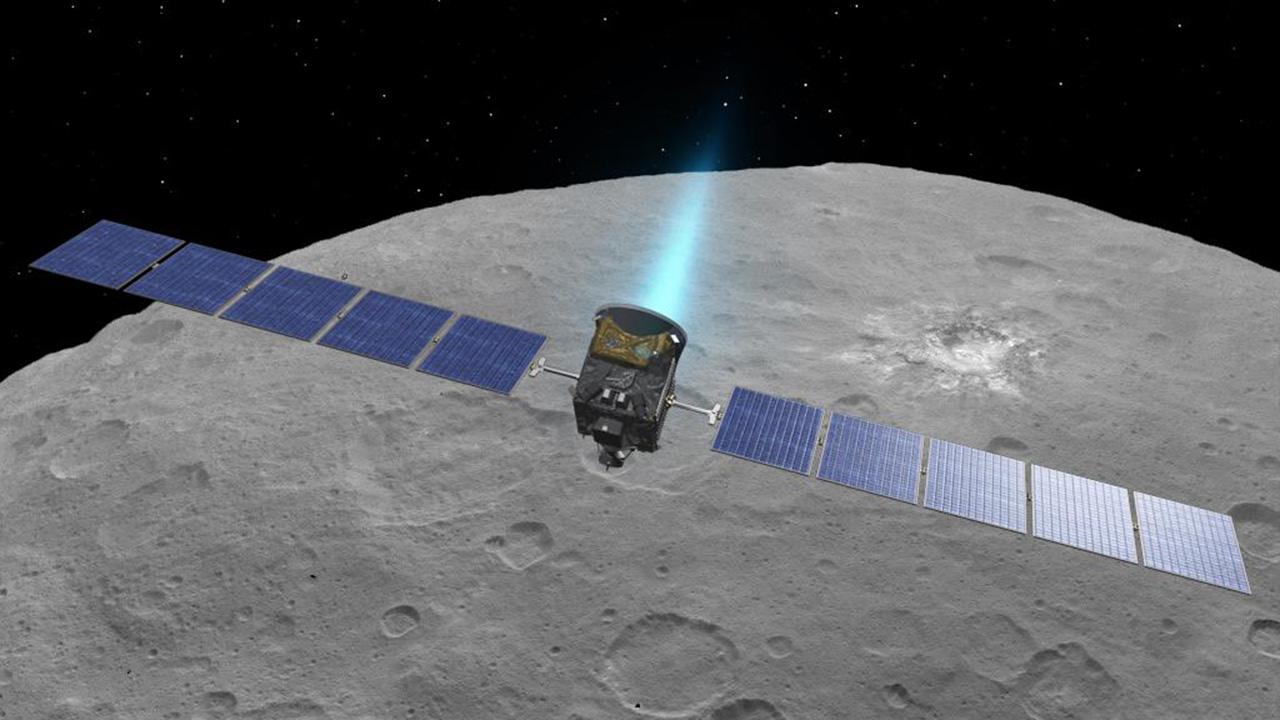
\includegraphics[width=0.6\columnwidth]{figures/dawn.jpg}
                        \end{figure}
                    \item Accurately captures the complex interaction of rotation and gravititational gradient
                \end{itemize}
            \item Translational and Rotational Motion is tightly coupled
                \begin{align*}
                    \dot{\vb{x}} &= \vb{v}, \\
                    \parenth{m_1 + m_2} \dot{\vecbf{v}} &= m_1 R_A \deriv{U}{\vecbf{z}_1} + m_2 R_A \deriv{U}{\vecbf{z}_2} + \vecbf{u}_f, \\
                    \dot{R} &= R S(\vb{\Omega}) , \\
                    J \dot{\vecbf{\Omega}} + \vecbf{\Omega} \times J \vecbf{\Omega} &= \vecbf{M}_1 + \vecbf{M}_2 + \vecbf{u}_m. 
                \end{align*}

	\end{itemize}
	\end{minipage}% end of left half of block
	\begin{minipage}{0.5\columnwidth}% right half of block
        \begin{itemize}
            \item Spacecraft is operating around \Emph{Itokawa}
            \begin{itemize}
                \item Potentially hazardous near Earth asteroid which crosses the Earth's orbit
                \item 25413 Itokawa, discovered in 1998, is an ellipsoid with axes \( 535 \times 294 \times 209 \si{\meter}\)
                \item Visited by Hayabusa in 2005 and samples returned to the Earth 
                \item Highest fidelity shape model allows for accurate simulation of sensor measurements
            \end{itemize}
        \end{itemize}
		\begin{figure}
			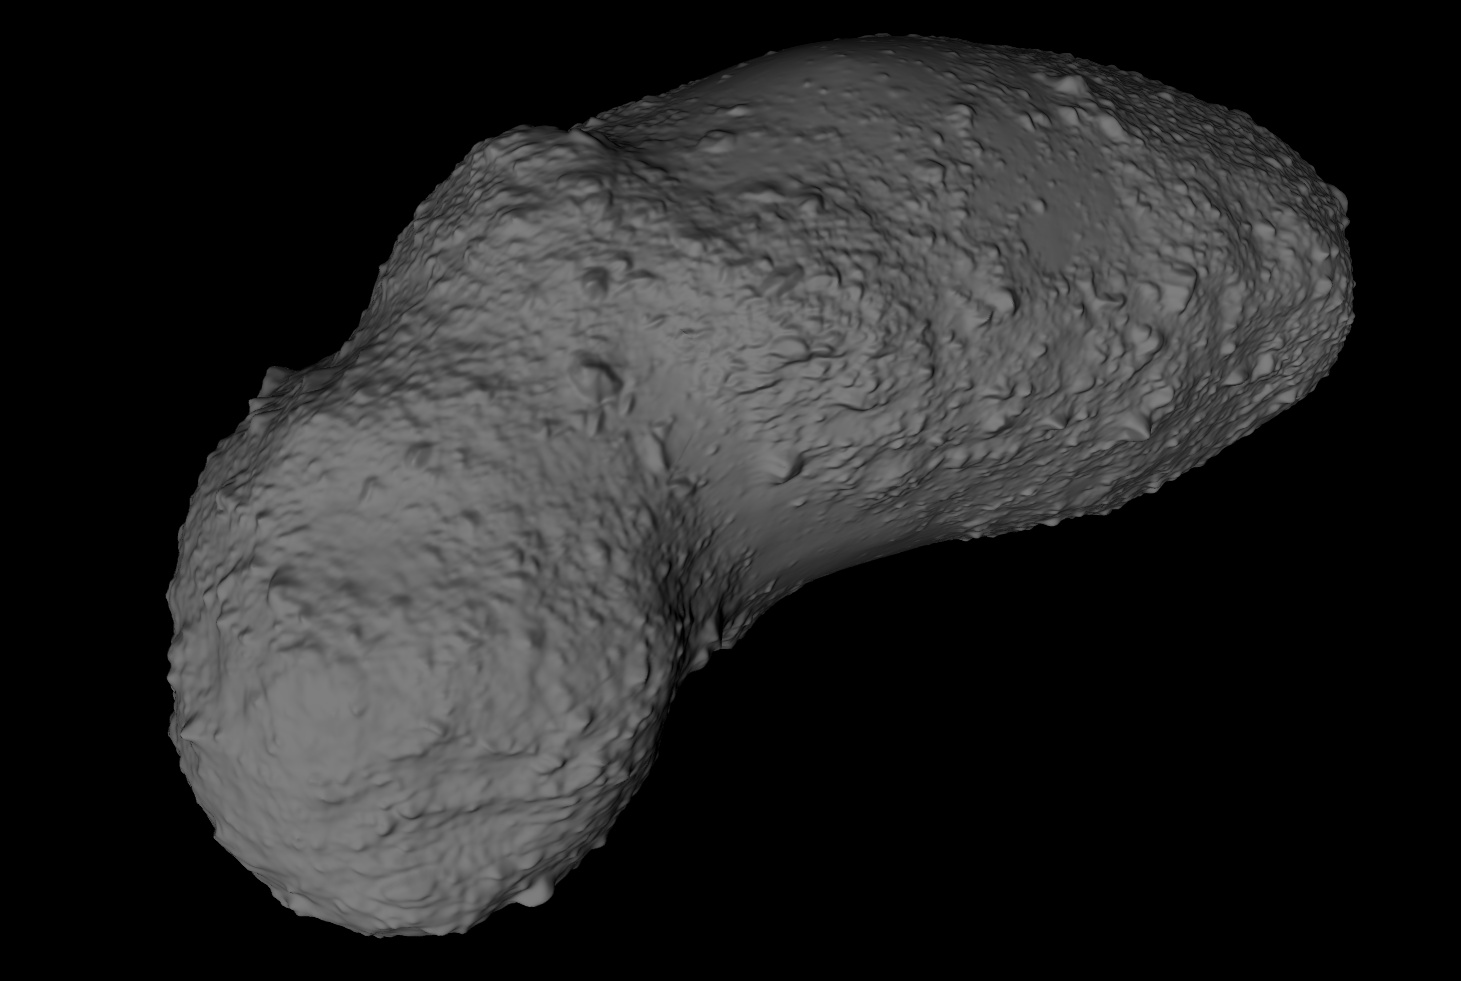
\includegraphics[width=0.7\columnwidth]{figures/itokawa.jpg}
			\caption*{Asteroid 25413 Itokawa}
		\end{figure}
	\end{minipage}%end of right half of block
\vspace{1.3cm}
\end{block} % end of structure block

\begin{block}{Shape model reconstruction from LIDAR} % results block
    \begin{minipage}[t]{0.5\columnwidth}
    \begin{itemize}
        \item Transfer between two periodic orbits of 4769 Castalia
        \begin{itemize}
            \item Thruster represents a current electric propulsion \( \approx \SI{600}{\milli\newton}\)
            \item Combining multiple iterations of the \Emph{rechability} computation allows for general transfers
        \end{itemize}
        \item Combining four iterations of the reachability set
        \begin{itemize}
            \item Each iteration of the reachability set enlarges the achievable states
            \item We choose a direction on the reachability set which lies closest to the target
            \[
                d = \sqrt{k_x \parenth{x_f - x_t }^2 + k_z \parenth{z_f - z_t }^2 + k_{\dot{x}}\parenth{\dot{x}_f - \dot{x}_t }^2 + k_{\dot{z}}\parenth{\dot{z}_f - \dot{z}_t }^2}
            \]
            \item This iterative approach avoids the difficulty in choosing accurate initial guesses for optimization
        \end{itemize}
    \end{itemize}
    \end{minipage}~
    \begin{minipage}[t]{0.5\columnwidth}
    \begin{itemize}
        \item \Emph{Optimal Control} is used to calculate the reachability set
            \[
            J = -\frac{1}{2} \left( \vecbf{x}(t_f) - \vecbf{x}_{n}(t_f)\right)^T Q \left( \vecbf{x}(t_f) - \vecbf{x}_{n}(t_f)\right) 
            \]
        \item Maximize the distance on the section using the low thrust propulsion
        \item Thruster magnitude is limited by physical system
        \[
            c(\vecbf{u}) = \vecbf{u}^T \vecbf{u} - u_m^2 \leq 0 
        \]
        \item Terminal constraints ensure intersection with the section
    \end{itemize}
        \begin{align*}\label{eq:terminal_constraints}
            \begin{split}
                m_1 &= y = 0  \\
                m_2 &= \parenth{\sin \phi_{1_{d}}} \parenth{ x_1^2 + x_2^2 + x_3^2 + x_4^2} - x_1^2 = 0 \\
                m_3 &= \parenth{\sin \phi_{2_{d}}} \parenth{ x_2^2 + x_3^2 + x_4^2} - x_2^2 = 0\\
                m_4 &= \parenth{\sin \phi_{3_{d}}} \parenth{ 2 x_3^2 + 2 x_3 \sqrt{x_4^2 + 2 x_4^2}} - x_3 - \sqrt{x_4^2 + x_3^2} = 0 
            \end{split}
        \end{align*}
    \end{minipage}

\begin{figure}[htbp] 
    \centering 
    \begin{subfigure}[htbp]{0.5\textwidth} 
        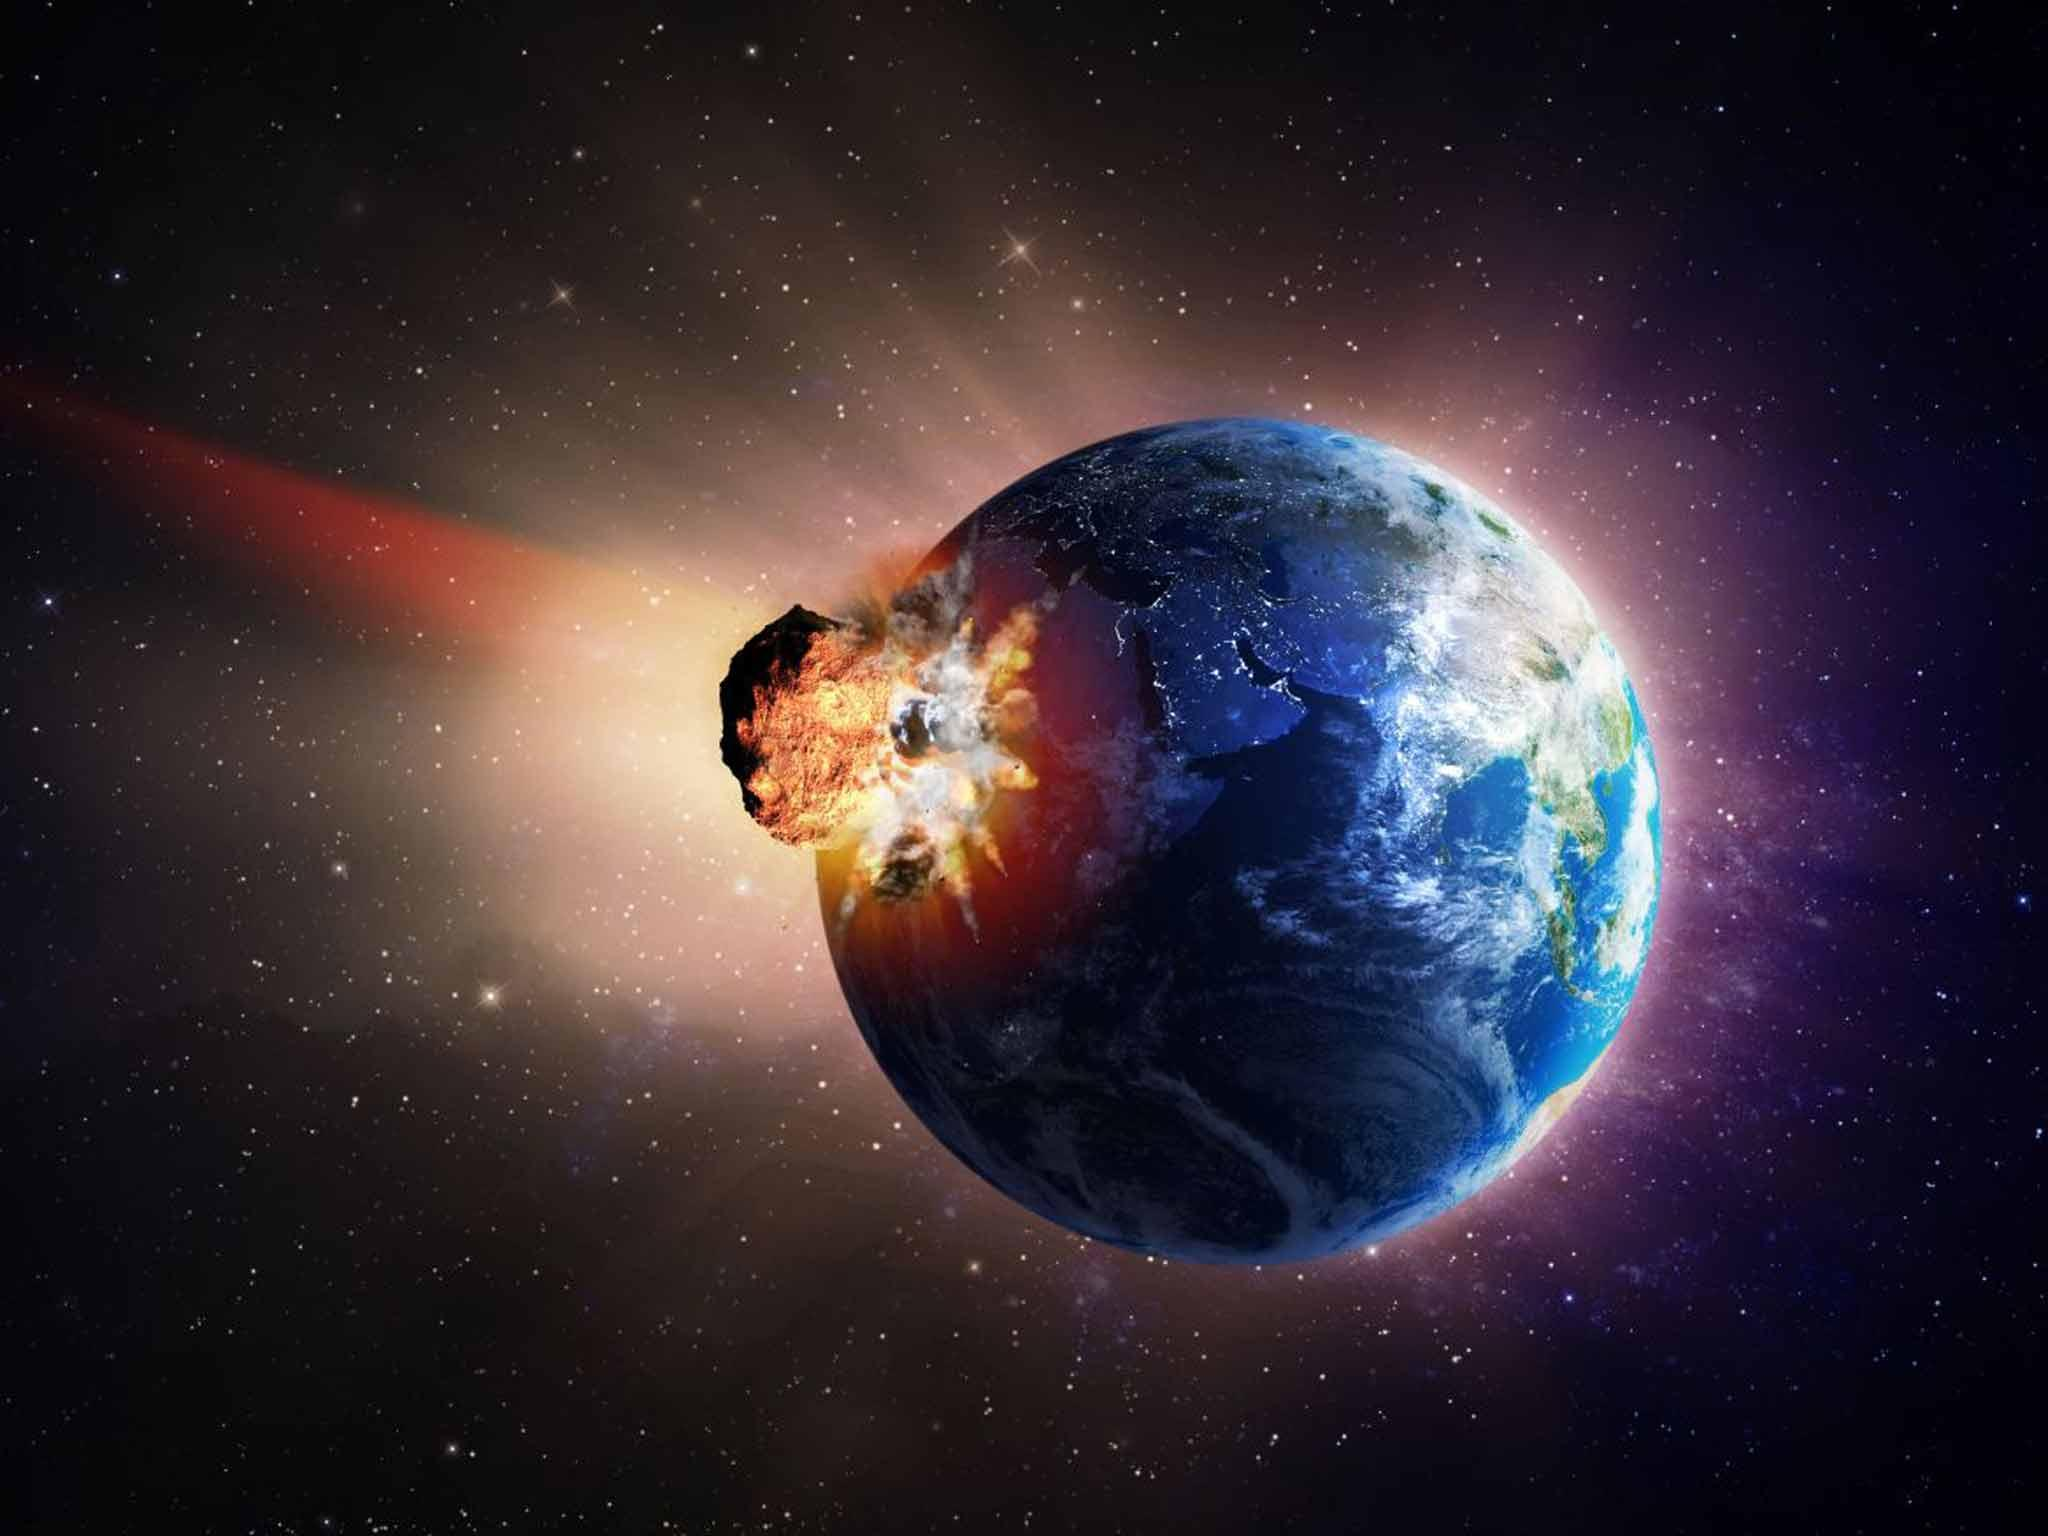
\includegraphics[width=\textwidth,draft]{figures/asteroid-alamy.jpg} 
        \caption{Equatorial Transfer Trajectory}
    \end{subfigure}~ %add desired spacing between images, e. g. ~, \quad, \qquad, \hfill etc. %(or a blank line to force the subfigure onto a new line) 
    \begin{subfigure}[htbp]{0.5\textwidth} 
        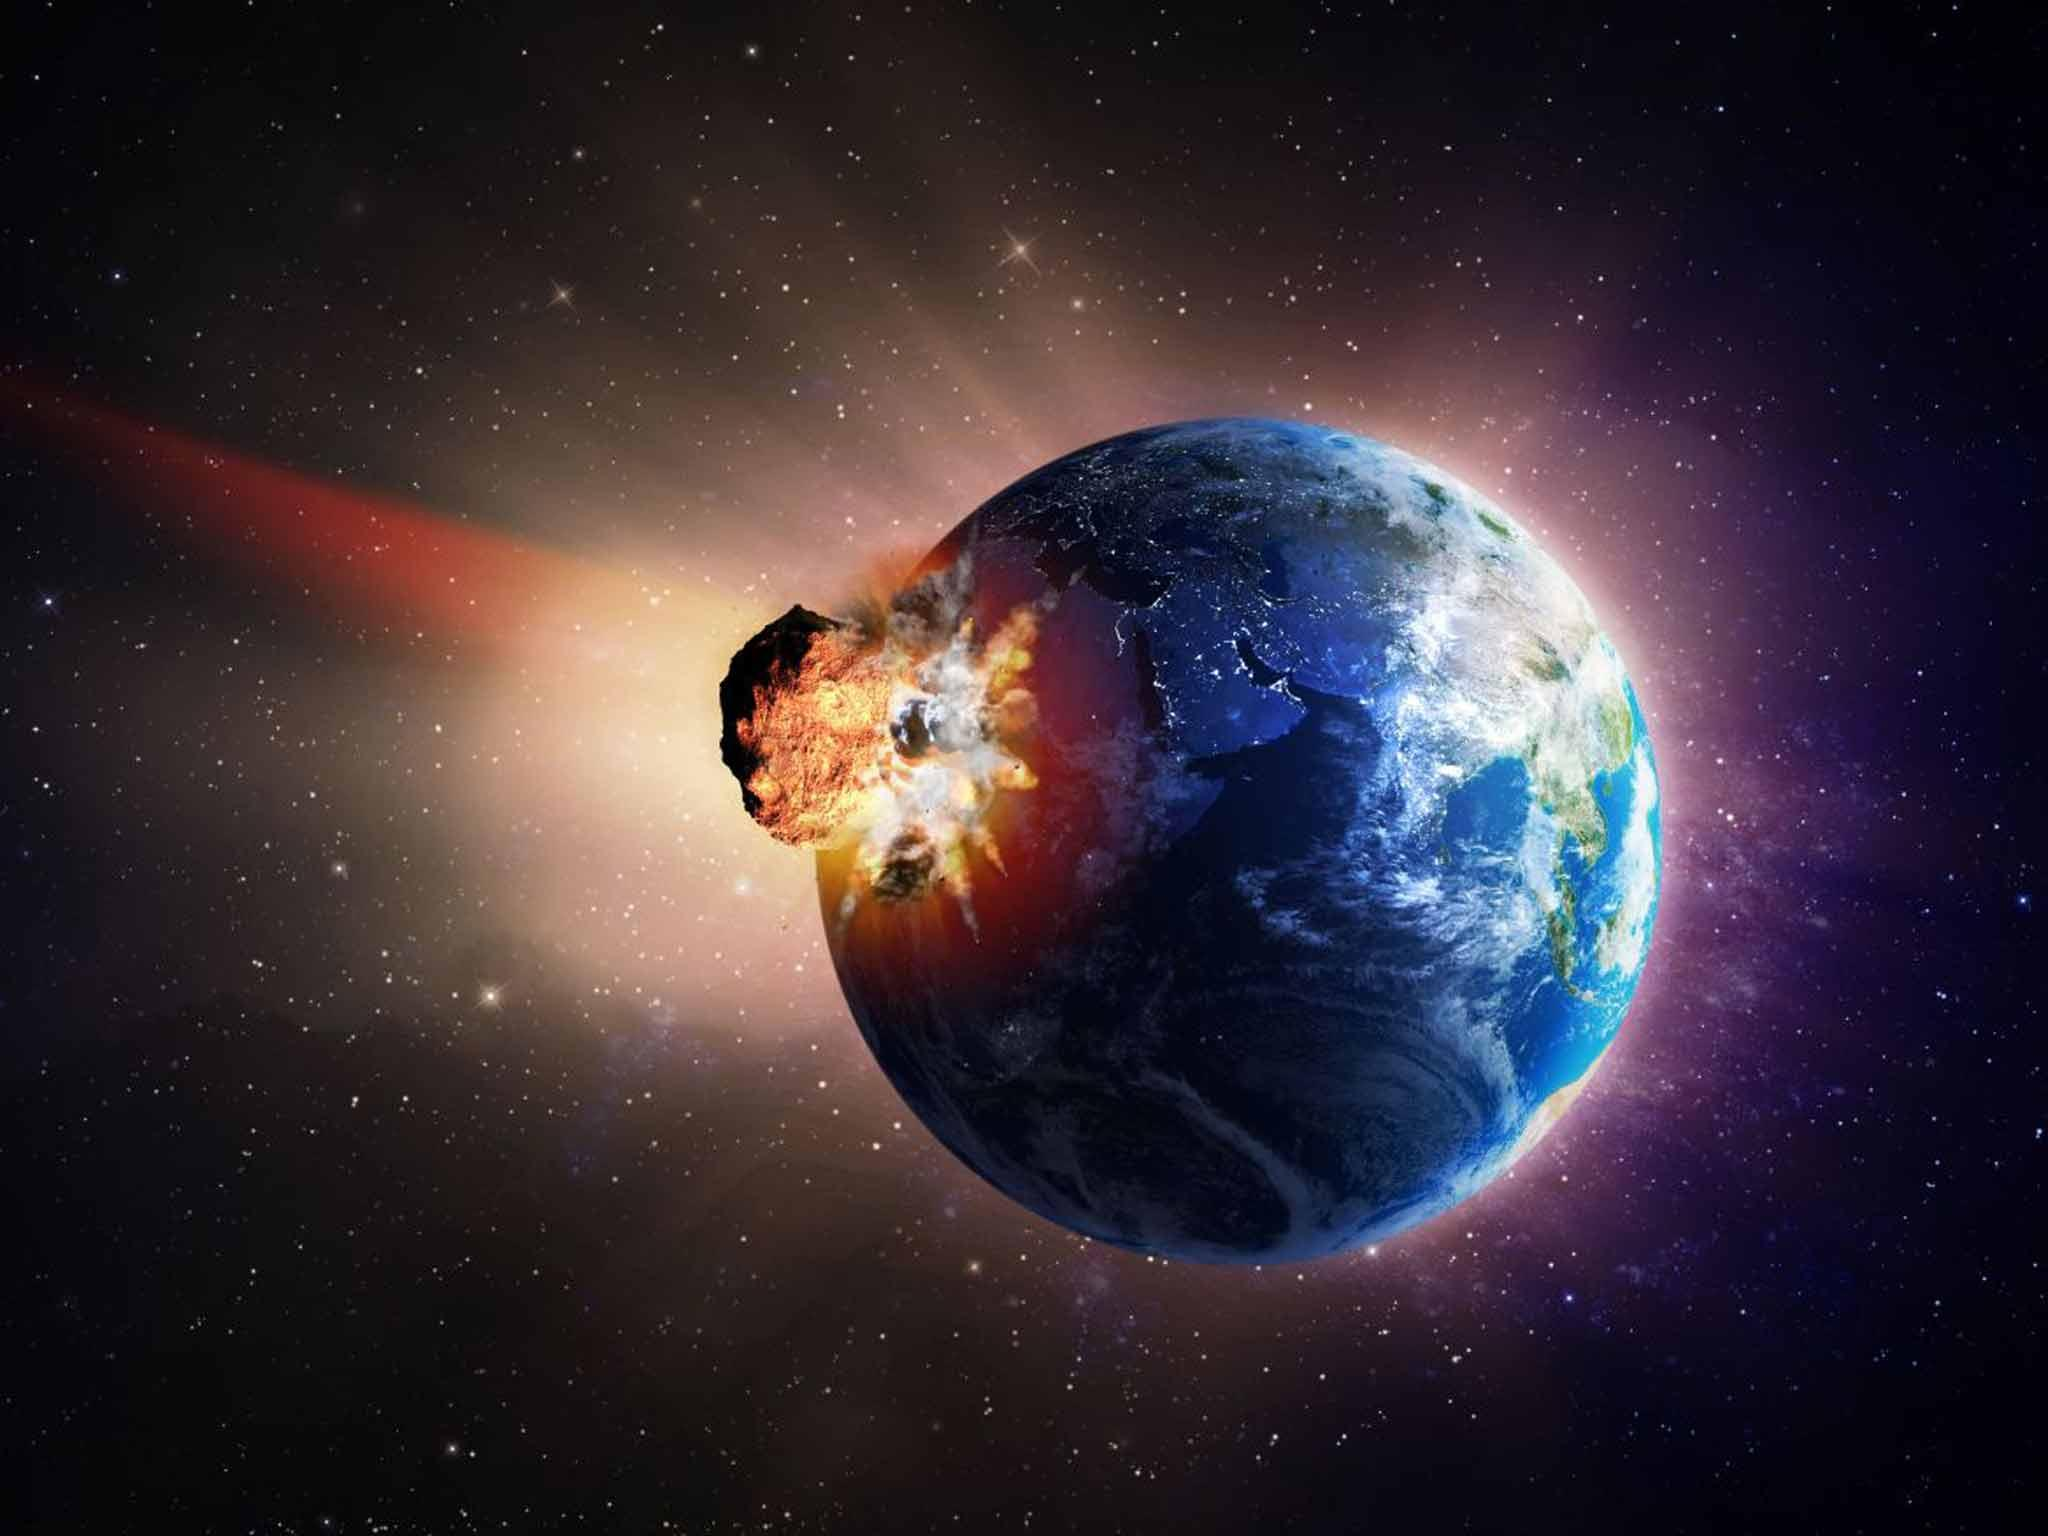
\includegraphics[width=\textwidth,draft]{figures/asteroid-alamy.jpg} 
        \caption*{3D Transfer Trajectory}
    \end{subfigure}
 
\end{figure}
    
\vspace{2cm}
\end{block} % end of results block
\end{column}


%-----------------------------------------------------------------------------------------
% THIRD (RIGHT) COLUMN
%---------------------------------------------------------------------------------------
\begin{column}{\onecolwidth} % third column start

\begin{block}{This is the third column environment} % results block
	\begin{itemize}
		\item Make sure to talk about how awesome your research is
	\end{itemize}
\end{block} % end of results block

\begin{block}{Conclusions} % conclusion
	\begin{itemize}
		\item Remind them about everything you already told them
		\item They should be quite amazed by this point
	\end{itemize}
\end{block} % conclusion
\end{column}  % third column end

\end{columns} % end of all columns in poster
\end{frame} % end of enclosing frame
\end{document}
